\documentclass{beamer}

\usefonttheme[onlymath]{serif}
\usepackage{subfig}
\usepackage{amsmath}
\usepackage{mathtools}

\title{Distributed Laplacian Solver}
\author{Rahul V}

\begin{document}

%1
\frame {
    \titlepage
}

%2
\frame {
    \frametitle{Problem Statement}
    \begin{itemize}
        \item
            Solve $Lx=b$ where $L=D-A$.
        \item
            Properties of $L$:
            \begin{enumerate}
                \item
                    Symmetric, diagonally dominant
                \item
                    Singular, Positive semi-definite
                \item
                    Sum of each row is $0$
            \end{enumerate}
        \item
            One sink: $b_{n} = -\sum_{i=1}^{n-1}b_{i}$
    \end{itemize}
}

%3
\frame {
    \frametitle{Approach: Random walk}
    \begin{itemize}
        \item
            Solve Data Collection Problem (DCP)
            \begin{itemize}
                \item[\textbullet]
                    Each node generates a packet with probability $\beta J_{u}$
                \item[\textbullet]
                    Random packet from queue and a random neighbor $v$ with
                    probability directly propotional to $w_{uv}$
                \item[\textbullet]
                    The packet is then transmitted to this neighbor
                \item[\textbullet]
                    Packets sunk at the sink immediately
            \end{itemize}
        \item
            At stationarity,
            $\eta^{T}(I - P) = \beta J^{T}$
            or
            $(\eta^{T}D^{-1})L = \beta J^{T}$ holds
        \item
            Ergodic iff $\beta < \beta^{*}$, and we have a lower
            limit for $\beta^{*}$. So we binary search on $\beta$.
        \item
            Scale and shift $x$ for canonical solution, i.e.,
            $<x, 1> = 0$
    \end{itemize}
}

%4
\frame {
    \frametitle{Status quo: Practical concerns}
    \framesubtitle{Testing}
    \begin{itemize}
        \item
            Guarantee by the algorithm:\\
            $|x_{u} - \hat{x_{u}}| < (\epsilon_{1} + \epsilon_{2})x_{u}$
            , whenever $\kappa < x_{u}d_{u}$
        \item
            Test set construction:
            \begin{itemize}
                \item[\textbullet]
                    $m =$ random from $[n - 1, n(n - 1)/2]$
                \item[\textbullet]
                    Generate Random MST with random weights in $[0, 100]$
                \item[\textbullet]
                    Generate random edges by selecting $2$ random nodes
                \item[\textbullet]
                    $b_{i}$ is chosen randomly from $[0, 1000]$
            \end{itemize}
    \end{itemize}
}

%5
\frame {
    \frametitle{Status quo: Practical concerns}
    \framesubtitle{Performance}
    \begin{itemize}
        \item
            $(\kappa, \epsilon_{1}, \epsilon_{2}) = (0.1, 0.1, 0.1)$
        \item
            Shared memory model with $4$ threads
        \item
            Fixed number of rounds ($O(nlogn)$), sampling from the start
    \end{itemize}
    \begin{figure}
        \centering
        \subfloat[Performance]{
            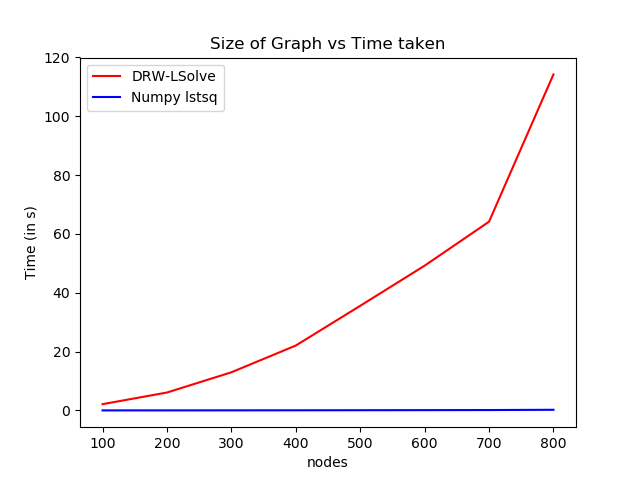
\includegraphics[height=5cm,width=5cm]{img/tcomp.png}
        }
        \subfloat[Accuracy]{
            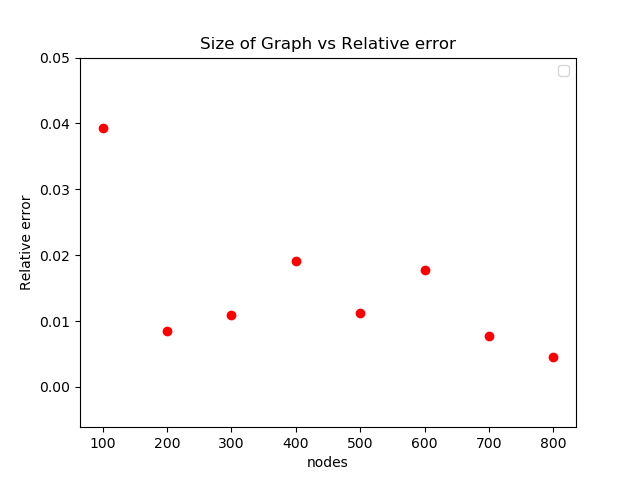
\includegraphics[height=5cm,width=5cm]{img/relerr.png}
        }
        \label{fig:plots}
    \end{figure}
}

%6
\frame {
    \frametitle{Near future}
    \begin{itemize}
        \item
            Use Message Passing instead of Shared memory model
        \item
            Graph partitioning to reduce communications, who should be at the
            boundary:
            \begin{itemize}
                \item[\textbullet]
                    Work as long as possible without need for checking queue
                \item[\textbullet]
                    Get very few packets in the first place
            \end{itemize}
    \end{itemize}
}

%7
\frame[c] {
    \centering \Huge \emph{Thank you}
}

\end{document}
